\hypertarget{a00011}{\subsection{Server.\-Lobby\-Server.\-Client\-Listener\-Thread Klassenreferenz}
\label{a00011}\index{Server.\-Lobby\-Server.\-Client\-Listener\-Thread@{Server.\-Lobby\-Server.\-Client\-Listener\-Thread}}
}
Klassendiagramm für Server.\-Lobby\-Server.\-Client\-Listener\-Thread\-:\begin{figure}[H]
\begin{center}
\leavevmode
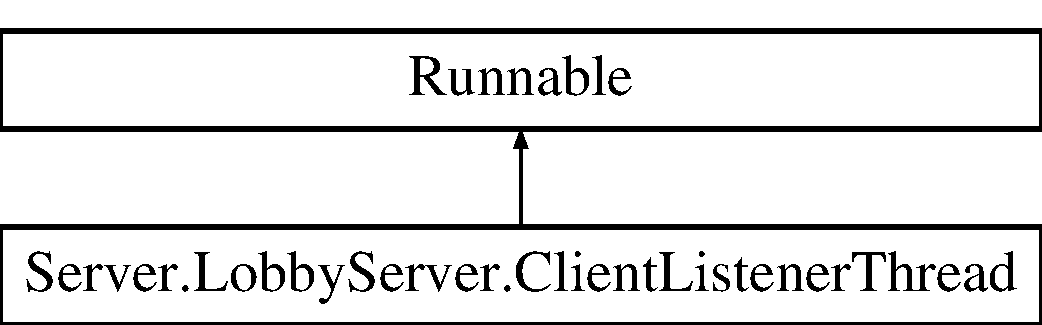
\includegraphics[height=2.000000cm]{a00011}
\end{center}
\end{figure}


\subsubsection{Ausführliche Beschreibung}
Der Thread auf eingehende Clientverbindungen, stellt diese her und instanziiert für jede Verbindung eine Klasse \hyperlink{a00073}{Player}. Dieser wird dann dem \hyperlink{a00054}{Lobby\-Server} übergeben. \begin{DoxyAuthor}{Autor}
Viktoria 
\end{DoxyAuthor}
